
\documentclass{article} % For LaTeX2e
\usepackage{iclr2026_conference,times}

% Optional math commands from https://github.com/goodfeli/dlbook_notation.
\input{math_commands.tex}

\usepackage{kotex}
\usepackage{booktabs}       % professional-quality tables
\usepackage{amsfonts}       % blackboard math symbols
\usepackage{nicefrac}       % compact symbols for 1/2, etc.
\usepackage{microtype}      % microtypography
\usepackage{xcolor}         % colors
\usepackage{amsmath}
\usepackage{colortbl}
\usepackage{hyperref}
\usepackage{url}
\usepackage{graphicx} % for \resizebox
\usepackage{float} % preamble에 추가
\usepackage{hyperref}
\input{iclr2026/preamble}

\definecolor{myred}{RGB}{255, 200, 200}     
\definecolor{myorange}{RGB}{255, 225, 180}  
\definecolor{myyellow}{RGB}{255, 255, 200}   

\title{HOIGS: Human-Object Interaction Gaussian Splatting from Monocular Videos}

 

\newcommand{\fix}{\marginpar{FIX}}
\newcommand{\new}{\marginpar{NEW}}
 
\begin{document}

\maketitle
\maketitle
\begin{figure}[H]
    \centering
    \includegraphics[width=\textwidth]{images/intro/intro.jpg}
    \vspace{-20pt}
    \caption{\textbf{Comparison between our method and previous approaches.}
    This figure compares rendering results between ExAvatar (\textcolor{blue}{\cite{moon2024expressive}}), a human-centric model, and Ex4DGS (\textcolor{blue}{\cite{lee2024fully}}), which uses a single motion field for all motions. ExAvatar reconstructs only humans, while Ex4DGS fails to represent contact in interaction scenarios, producing artifacts and noise around contact regions. }
    \label{fig:teaser}
\end{figure}
\vspace{-10pt}
\input{iclr2026/section/0_Abstract}
\input{iclr2026/section/1_Introduction}
\input{iclr2026/section/2_Relatedwork}
\input{iclr2026/images_tex/main_fig}

\section{Method}
% 
% method 개요 설명
%우리는 사람과 객체의 deformation을 각각 독립적으로 모델링한 뒤, HOI 모듈을 통해 상호작용에 따른 변형을 반영하여 최종적으로 장면을 재구성한다. 먼저 객체의 deformation은 Cubic Hermite Spline을 통해 추정한다. 사람의 deformation은 HexPlane feature를 기반으로 하며, 시간에 대해 불변한 spatial feature를 활용하여 canonical space에 정의된 T-pose의 texture를 학습하고, 이후 Linear Blend Skinning(LBS)을 통해 각 world space로 deformation을 적용한다. 이러한 deformation baseline을 통해 사람과 객체를 각각 모델링하며 각 프레임에 대한 대략적인 위치를 추정한 뒤, 그로부터 motion feature를 추출한다. 마지막으로, 추출된 human과 object feature를 HOI 모듈에 입력하여 두 객체 간 상관관계에 따른 변형을 고려하고, 이를 통해 최종적으로 interaction 장면에서의 사람과 객체의 위치를 결정한다. 
As shown in Fig. \textcolor{blue}{~\ref{figure_main_method}}, we reconstruct the scene by independently modeling the deformations of humans and objects, and then incorporating interaction-aware transformations through the HOI module. Object deformations are estimated using a Cubic Hermite Spline (CHS). Human deformations are based on hexplane features, where time-invariant spatial features are used to learn the texture of the canonical T-pose, and Linear Blend Skinning (LBS) is subsequently applied to deform the canonical representation into each world space. Using these deformation baselines, we independently model humans and objects and estimate their approximate positions for each frame, from which motion features are extracted. Finally, the extracted human and object features are fed into the HOI module, which accounts for interaction-driven transformations and determines the final positions of humans and objects in the reconstructed interaction scene.
\subsection{Object deformation}
% 우리는 diffusion prior와 SDS loss를 적용하여 전체 시퀀스를 대표하는 프레임에서 객체를 재구성한다. 재구성된 객체는 각 키프레임의 카메라 파라미터를 이용해 warping을 수행함으로써, 해당 키프레임의 3D Gaussian을 초기화한다% .
%Diffusion prior를 통해 생성된 3D Gaussian은 실제 물체의 형상과 다소 차이가 있을 수 있다. Diffusion은 그럴듯한 이미지를 기반으로 3D shape을 생성할 수 있으나, 실제 물체의 형상을 정확하게 복원하지는 못한다. 이에 우리는 diffusion 기반으로 생성된 초기 3D shape을 실제 물체의 형상 및 기하 정보와 정합시키기 위해, explicit한 3D Gaussian deformation 모델을 도입% 한다.
%key frame들로 warping된 Gaussian $G_k$의 mean 값 $\mathbf{m}$과 color 값만을 추출하고, 나머지 3D Gaussian 파라미터는 identity 값으로 초기화한다. 우리는 key frame에서 새롭게 정의된 mean과 color를 기반으로 object의 3D Gaussians을 구성하고, 이를 통해 object의 deformation을 모% 델링한다.
%Object의 시간에 따른 연속적인 움직임을 표현하기 위해, 각 Gaussian의 mean 값을 제어점 기반의 곡선으로 모델링한다. 이를 위해 Cubic Hermite Spline 기반의 함수 $CHP(t, \mathbf{m})$를 정의하고, 시간 $t$에서의 object Gaussian의 위치 $M(t)$를 다음과 같이 추정한다:
% $M(t)=CHP(t, m)$ 
% 여기서 $\mathbf{m} = \left{ \mathbf{m}_k \mid \mathbf{m}k \in \mathbb{R}^3 \right}{k \in [0, N_c - 1]}$는 key frame들의 mean 위치들로 구성된 learnable한 제어점 집합이며, $N_{key}$는 제어점의 개수를 나타낸다.
% $CHP(t, m)$은 다음과 같이 수식화된다:
%수식
% notation설명.
%$m_{\lfloor t_s \rfloor}$는 $\lfloor t_s \rfloor$번째 key frame에 해당하는 3D Gaussian의 mean 값을 의미한다.
%기존의 spline 정의에서 tangent는 단순히 보간을 위한 기울기로 사용되지만, 우리는 이를 velocity로 해석하여 motion feature로 활용한다. 즉, 각 Gaussian mean의 시간에 따른 위치 변화율을 velocity vector로 정의하고, 이를 임베딩함으로써 객체의 motion feature를 구성한다. 이렇게 얻어진 velocity 기반 motion feature는 객체의 동적인 움직임을 보다 효과적으로 표현할 수 있다.
% Key frame 사이의 위치 파라미터 $m$은 각 key frame에 존재하는 Gaussian의 위치 $m_k$를 기반으로 Spline을 이용해 추정된다. 학습되는 Gaussian들은 key frame에 대응되는 Gaussian들로, key frame 사이의 Gaussian은 추정된 후 렌더링되고, 손실 함수를 통해 계산된 gradient가 역전파되어 해당 key frame의 Gaussian 파라미터가 업데이트된다.
% Gaussian 파라미터 중 rotation과 opacity는 시간에 따라 변화하는(time-dependent) 파라미터로 설정하였다. Rotation은 각 key frame에서의 Gaussian rotation 값을 기반으로 Spherical Linear Interpolation(Slerp)을 적용하여 시간에 따른 연속적인 변화를 모델링하였다. Opacity는 물체의 움직임에 따라 발생하는 occlusion 영역을 반영할 수 있도록 time 값에 따라 변화하도록 설계하였다. 한편, scale 파라미터는 모든 key frame에서 대응되는 Gaussian들에 대해 동일한 값으로 고정하였다.
We apply a diffusion prior with SDS loss to reconstruct the object from a representative frame of the entire sequence. The reconstructed object is then warped using the camera parameters of each keyframe to initialize the corresponding 3D Gaussians.
However, the 3D Gaussians generated through the diffusion prior may differ from the actual object geometry. While diffusion models can generate plausible 3D shapes from images, they often fail to precisely recover the true object structure. To address this, we introduce an explicit 3D Gaussian deformation model that aligns the diffusion-based initialization with the actual object geometry and structural information.
From the warped Gaussians $G_k$ of each keyframe, we extract each Gaussian's mean and color value, while initializing the remaining 3D Gaussian parameters with identity values. Based on the redefined mean and color from the keyframes, we construct the object’s 3D Gaussians and use them to model the object deformation.
To represent the continuous motion of the object over time, we model the mean values of each Gaussian as control-point-based curves. Specifically, we define a Cubic Hermite Spline function $CHS(t, \mathbf{m})$, and estimate the position of an object Gaussian at time $t$, denoted as $M(t)$, as follows:
\[
M(t) = CHS(t, \bold{m}), \tag{1}
\]
where $\bold{m} = \left\{ m_k \mid m_k \in \mathbb{R}^3 \right\}_{k \in [0, N_{key} - 1]}$ is a learnable set of control points representing the mean positions of the Gaussians at each key frame, and $N_{key}$ denotes the number of key frames. $CHS(t, \mathbf{m})$ is formulated as

\begin{equation}
\begin{aligned}
CHS(t, \mathbf{m}) &= (2t_r^3 - 3t_r^2 + 1)m_{\lfloor  t_s  \rfloor} + (t_r^3 - 2t_r^2 + t_r)\tau_{\lfloor t_s \rfloor  } \\
&\quad + (-2t_r^3 + 3t_r^2)m_{\lfloor t_s  \rfloor + 1} + (t_r^3 - t_r^2)\tau_{\lfloor t_s \rfloor  + 1}, 
\end{aligned} \tag{2}
\end{equation}

where $t_r = t_s - \lfloor t_s  \rfloor $, $t_s = t_n (N_{key} - 1)$, $t_n = \frac{t}{N_f - 1}$ and $N_f$ denotes the number of all frames.
$m_{\lfloor t_s \rfloor}$ denotes the mean of the 3D Gaussians corresponding to the $\lfloor t_s \rfloor$-th key frame.

In the standard formulation, $\tau_{\lfloor t_s \rfloor}$ represents the tangent vector with respect to the means of the surrounding Gaussians, which is typically approximated as $\tau_{\lfloor t_s \rfloor} = \tfrac{1}{2}\left(m_{\lfloor t_s \rfloor+1} - m_{\lfloor t_s \rfloor-1}\right)$. Instead of using this fixed approximation, we reinterpret $\tau_{\lfloor t_s \rfloor}$ as a \textit{velocity vector} and employ it as a learnable parameter. By embedding this velocity, we construct motion features that better capture the dynamic behavior of objects over time.

The position parameter $\bold{m}$ between key frames is estimated via spline interpolation using both the Gaussian positions $m_k$ at the key frames and the corresponding velocity vectors $\tau_{ \lfloor k \rfloor }$. Only the Gaussians at the key frames are directly optimized during training. Once the intermediate Gaussians are estimated and rendered, the resulting gradients from the loss function are backpropagated to update the parameters of the corresponding key frame Gaussians.
Among the Gaussian parameters, rotation and opacity are defined as time-dependent variables. The rotation parameter is modeled using Spherical Linear Interpolation based on the Gaussian rotations at each key frame, enabling smooth transitions over time. The opacity parameter varies with time to account for occluded regions caused by object motion. In contrast, the scale parameter is kept constant across all corresponding Gaussians at different key frames.
\subsection{Human deformation}
We model human deformation using hexplane features. 
Specifically, we adopt time-invariant spatial features $f$ from hexplane to learn the texture of the canonical T-pose mesh $T_c$ in the canonical space. The features $f$ are processed by an MLP head $\psi$ to learn the Gaussian properties in the canonical space. This representation serves as the baseline for human deformation. The canonical human representation is then deformed into the posed world space using Linear Blend Skinning (LBS) as follows:
\begin{equation}
\psi_h(f(T_c)) = (c, o, \Delta P_c, R, S, W), \tag{3}
\end{equation}
\begin{equation}
P_{def} = \alpha * LBS(P_c , \theta, W), \tag{4}
\end{equation}
where $\theta$ denotes the set of SMPL-X pose parameters and $\alpha$ is a learnable scale parameter for human pose. 
Equation (3) extracts the Gaussian properties (color $c$, opacity $o$, position offset $\Delta P_c$, rotation $R$, scale $S$ and skinning weights $W$) from the canonical hexplane features, 
while Equation (4) applies the LBS function to obtain the deformed positions $P_{def}$ of the Gaussians in the posed space. 

To ensure that the reconstructed human representation matches the actual geometry, 
we further apply a depth supervision loss:
\begin{equation}
\mathcal{L}_{depth} = \left\| D_{render} - D \right\|_1, \tag{5}
\end{equation}
where $D_{render}$ is the rendered depth map from the deformed Gaussians and $D$ is the depth obtained from an off-the-shelf metric depth estimation model and further scaled using the COLMAP point cloud. 
This depth-guided supervision constrains the learnable scale parameter $\alpha$ and improves geometric fidelity in the reconstructed human shape.

\subsection{HOI module}
\textbf{Feature Extraction.} We extract time-varying features from both humans and objects to learn their interactions. For humans, instead of relying on time-invariant texture features from the canonical space, we utilize time-varying features from hexplane. Furthermore, since it is not possible to know in advance which body parts are involved in object interactions, we divide the human body into 16 parts and extract hexplane features for each part.

For objects, the features are derived from the velocity embeddings associated with each keyframe in the deformation process, which capture the local motion information at those frames. In addition, we embed learnable parameters for each keyframe to represent latent motion characteristics that cannot be fully captured by velocity alone. These velocity vectors and learnable parameters are then projected together with the corresponding time values, enabling the construction of object motion features. This formulation allows us to obtain continuous motion features for objects across all frames, rather than being limited to discrete keyframes.

\textbf{HOI module.} The proposed HOI module takes time-varying features of humans and objects as inputs and explicitly models their interactions. 
Let the human and object features be denoted as $F_{\text{Human}}$ and $F_{\text{Object}}$. 
To capture interdependencies between the two, we apply \textit{mutual attention}, where queries, keys, and values are defined as:
\begin{equation}
Q_h = F_{\text{Human}}W_h^Q,\;\; K_o = F_{\text{Object}}W_o^K,\;\; V_o = F_{\text{Object}}W_o^V, \tag{6}
\end{equation}
\begin{equation}
Q_o = F_{\text{Object}}W_o^Q,\;\; K_h = F_{\text{Human}}W_h^K,\;\; V_h = F_{\text{Human}}W_h^V. \tag{7}
\end{equation}

Cross-attention is then performed in both directions, from human to object and from object to human, while incorporating a distance mask $B$ into the attention computation:
\begin{equation}
A_{h \leftarrow o} = \text{softmax}\!\left(\tfrac{Q_hK_o^\top}{\sqrt{d}} + B\right),\quad
A_{o \leftarrow h} = \text{softmax}\!\left(\tfrac{Q_oK_h^\top}{\sqrt{d}} + B^\top\right). \tag{8}
\end{equation}

This process yields updated features $F'_{\text{Human}}$ and $F'_{\text{Object}}$ that embed interaction cues. 
Finally, $F'_{\text{Human}}$ is used to regress $\Delta$SMPL-X refinements (body pose, hand pose, translation), while $F'_{\text{Object}}$ is used to predict $\Delta G_{\text{object}}$, i.e., corrections for Gaussian-based object motion. 
In this way, the HOI module augments the baseline deformations (hexplane+LBS for humans and CHS for objects) with interaction-aware adjustments, enabling accurate reconstruction of human--object interaction scenes.

\subsection{Optimization}
% Canonical space에 정의된 T-pose 형태의 human Gaussian, 배경 Gaussian, 그리고 움직이는 객체에 대한 dynamic motion을 공동으로 최적화함으로써, human-object interaction 상황을 효과적으로 재구성한다. 우리는 기존 Human Gaussian Splatting 방법과 유사하게, 각 프레임에 대해 SMPL 파라미터를 regression하고, 모든 프레임에 공통으로 대응되는 T-pose 형태의 human canonial space에 정의한다. 이 canonial human을 기반으로 3D Gaussian 파라미터는 feature plane과 MLP를 통해 추정되며, 해당 파라미터는 texture가 표현된 공간을 구성한다. 이후 각 프레임의 회귀된 SMPL 파리미터를 바탕으로, LBS(Linear Blend Skinning)를 통해 canonical Gaussian들이 해당 프레임으로 deformation된다. 우리는 ExAvatar에서 영감을 받아, body shape뿐만 아니라 얼굴과 손의 표현까지 확장하기 위해 SMPL-X 모델을 사용하였다. 배경은 3D Gaussian Splatting 기반으로 표현된다.


% We reconstruct the final human-object interaction scenario by jointly optimizing the T-pose Gaussians defined in a canonical space, background Gaussians, and dynamic motion modeling for moving objects. Similar to existing human Gaussian Splatting approaches\cite{moreau2024human, li2024animatable, kocabas2024hugs, moon2024expressive, hu2024gauhuman, qian20243dgs}, we regress the SMPL parameters\cite{loper2023smpl} for each frame and define a canonical T-pose human shared across all frames. The 3D Gaussian parameters in the canonical space are predicted using a feature plane and an MLP, forming a textured space. These canonical Gaussians are then deformed to each frame using the regressed SMPL parameters via Linear Blend Skinning (LBS)\cite{loper2023smpl}. Inspired by ExAvatar\cite{moon2024expressive}, we adopt SMPL-X\cite{pavlakos2019expressive} to represent not only the body shape but also fine-grained facial and hand motions. The background is separately modeled using standard 3D Gaussian Splatting\cite{kerbl20233d}.

% 방금 언급한 human과 backgroud에 대한 모델, 그리고 object가 함께 최적화 되어지는 모습을 보이기!
% 사용된 loss들 전부 언급하고, loss를 통해 3D Gaussian들이 어떻게 global minimum을 찾아가는지를 기입

% 최적화 과정은 각가 독립적으로 분리되는 것이 아닌, 한번에 1-stage 로 함께 학습이 진행된다.
% 우리는, 객체, 인간, 배경을 동시에 모델링한다.
% 배경은 일반적인 3DGS( 3d gaussian splatting )을 사용하여, 모델링이 되었다.
% 학습에는 객체와 사람 영역 마스킹을 통해, 배경만을 분리하여, 정적 가우시안 배경이 photometric loss 를 통해 학습되었다.
% 사람 모델링의 경우, 기존에 존재하는 일반적인 접근 방법처럼, feature plane 기반 가우시안 모델링을 하였으며, 객체와 함께 상호작용하는 자연스러운 모델링을 위해, SMPL-X 기반 모델 아바타 모델을 사용하였다.
% 전 프레임에 대해, SMPL-X 파라미터를 추출하고, Canonical T-pose human avatar 를 정의해, LBS 변환을 통해 각 프레임에 변형시켰다.
% 학습 과정에는 가우시안 랜더러를 통해 나온 결과와 인간 영역을 비교하는 이미지 손실 기반 (SSIM,LPIPS,L1) 손실이 사용되었다. 자세한 내용은 부록에 기술하였다.
% \textbf{객체 시작 최적화}
% 객체는 SDS Loss 를 사용해 객체 모델링이 되었다. 객체 모델링에 있어서, 전체 프레임에서 객체를 마스킹을 통해 분리하고, 해당 객체를 diffusion을 통해 고해상도 3d 모델링을 한다.  학습에서 특정 카메라 뷰를 제한해 optimazation 과정이 안정화 되도록 하였다.

For background modeling, we employ the standard 3D Gaussian Splatting (3DGS) technique. During training, we isolate the background by masking out the object and human regions, allowing the static Gaussian background to be optimized using a photometric loss. For human modeling, we regress the SMPL parameters (\textcolor{blue}{\cite{loper2023smpl}}), and incorporate an SMPL-X-based avatar model to ensure natural interaction with the object. For each frame, we extract the SMPL-X parameters and define a canonical T-pose human avatar. This canonical avatar is then deformed to match each frame using LBS. During training, image-based loss metrics such as SSIM, LPIPS, and L1-norm were utilized to compare the Gaussian renderer's output with the human region in the image.

\textbf{Object Motion Optimization}
% 객체 모션 모델링
% 3차 스플라인(CHS)을 사용해 위치 보간을 위한 연속성을 보장했다. ~

We model the motion of objects using CHS to ensure continuity in position interpolation. A CHS is a piecewise cubic polynomial that is defined by both the positions and the first derivatives (tangents) at key points in time. By specifying the starting and ending slopes for each spline segment, CHS guarantees smooth transitions between key frames, maintaining continuity not only in the object’s position but also in its velocity. In other words, the object’s trajectory over time remains continuous and smooth, without abrupt jumps or changes in speed. This property is crucial for accurately modeling temporal motion in a realistic and stable manner.

\textbf{Integrated Optimization}
% 통합 최적화
We train our model using an integrated optimization objective that combines multiple loss terms. Specifically, the overall loss function is formulated as:
\[
\mathcal{L} = \gamma \, \mathcal{L}_{\text{object motion}} + \beta \, \mathcal{L}_{\text{human}} + \sigma \, \mathcal{L}_{\text{scene}} + \mathcal{L}_{\text{depth}}, \tag{9}
\]
where $\mathcal{L}_{\text{object motion}}$, $\mathcal{L}_{\text{human}}$, and $\mathcal{L}_{\text{scene}}$ are the loss components for the object's motion, the human-related factors, and the scene context, respectively. Here, $\gamma$, $\beta$, and $\sigma$ are hyperparameters that control the relative weight of each loss term during training. By tuning these hyperparameters, we balance the influence of each component on the training objective. This integrated optimization approach ensures that the model simultaneously accounts for object motion accuracy, human interaction plausibility, and scene consistency during learning.

\section{Experiments}

\subsection{Implementation Details}
We use ExAvatar (\textcolor{blue}{\cite{moon2024expressive}}) as the baseline human rendering model, and all hyperparameters are kept identical to those used in ExAvatar. For object deformation using splines (\textcolor{blue}{\cite{ahlberg2016theory, de1978practical}}), we fix the time interval to 4 for all scenes. Training is conducted using an NVIDIA H100 GPU, taking approximately 5 hours per scene.
\vspace{-5pt}
\subsection{Datasets}
\textbf{HOSNeRF dataset (\textcolor{blue}{\cite{liu2023hosnerf}}).} We use the monocular dynamic-scene dataset HOSNeRF, which captures human–object interaction scenarios. The dataset comprises recordings in six indoor and outdoor locations with six subjects interacting with objects within a single scenario. Each sequence contains 300–400 frames. For evaluation, we uniformly select 16 frames per sequence for testing and use the remaining frames for training, following HOSNeRF.

\textbf{BEHAVE dataset (\textcolor{blue}{\cite{bhatnagar2022behave}}).} We use the BEHAVE multi-view RGB-D human–object interaction dataset, but adapt it to a monocular setting by selecting a single fixed camera from the four static viewpoints for each sequence. Specifically, we curate 9 sequences covering four distinct indoor environments, five subjects, and four objects. From each sequence’s raw video, we uniformly sample 300 frames. For evaluation, we uniformly select 16 frames per sequence for testing and use the remaining frames for training 

\textbf{ARCTIC dataset (\textcolor{blue}{\cite{fan2023arctic}}).} We use the ARCTIC hand–object interaction dataset and extend comparisons to hand–object baselines. Since HOIGS is human-centric rather than hand-only, we evaluate only sequences where the full body is visible. Specifically, we use sequences of one subject interacting with four objects. Each monocular sequence (≈600 frames) is split by uniformly sampling 16 frames for testing and using the rest for training.


\begin{figure*}[t]
    \centering
    \includegraphics[width=\linewidth]
    {iclr2026/images/qualitative_main/ALL/qual_hosnerf.pdf}
    \footnotesize
    % set column padding 
    \setlength{\tabcolsep}{0pt}
    \begin{tabular}{@{\hspace{6mm}}c@{\hspace{9mm}}c@{\hspace{4mm}}c@{\hspace{3mm}}c@{\hspace{3mm}}c@{}}
        Ground Truth &
        HOIGS (Ours) &
        \makecell{ExAvatar\\(\textcolor{blue}{\cite{moon2024expressive}})} &
        \makecell{Ex4DGS\\(\textcolor{blue}{\cite{lee2024fully}})} &
        \makecell{D3DGS\\(\textcolor{blue}{\cite{yang2024deformable}})}
    \end{tabular}

    \caption{
    Qualitative comparison of reconstructed rendered view results on the HOSNeRF dataset.
    We display the full-frame (top) rendering and a zoom-in (bottom) of the red Region of Interest (ROI).
    }
    \vspace{-4mm}
    \label{fig:visual_HOSNeRF}
\end{figure*}


% \begin{figure*}[t]
%     \centering
%     \includegraphics[width=\linewidth]
%     {iclr2026/images/qualitative_main/ALL/qual_hosnerf.pdf}
%     \footnotesize
%     \begin{tabular}{ccccc}
%     Ground Truth &
%     HOIGS (Ours) &
%     \makecell{ExAvatar\\(\textcolor{blue}{\cite{moon2024expressive}})} &
%     \makecell{Ex4DGS\\(\textcolor{blue}{\cite{lee2024fully}})} &
%     \makecell{4DGS\\(\textcolor{blue}{\cite{wu20244d}})}
%     \end{tabular}
%     \caption{
%     Qualitative comparison of reconstructed rendered view results on the HOSNeRF dataset.
%     We display the full-frame (top) rendering and a zoom-in (bottom) of the red Region of Interest (ROI).
%     }
%     \vspace{-4mm}
%     \label{fig:qualitative_sota}
% \end{figure*}


% \begin{figure*}[t]
%     \centering
%     \includegraphics[width=\linewidth]{fig/qualitative_main/All/qual_hosnerf_pdf_cropped.pdf}
%     \small
%     \begin{tabular}{ccccc}
%         \hspace{0.3em} Ground Truth \hspace{5em} &
%         HOIGS (Ours) \hspace{5em} &
%         ExAvatar \hspace{5em} &
%         Ex4DGS \hspace{5em} &
%         E\text{-}D3DGS
%     \end{tabular}
%     \vspace{-5mm}
%     \caption{
%     Qualitative comparison of reconstructed rendered view results on the HOSNeRF dataset.
%     We display the full-frame (top) rendering and a zoom-in (bottom) of the red Region of Interest (ROI).
%     }
%     \label{fig:qualitative_sota}
% \end{figure*}


  

\begin{figure*}[t]
    \centering
    \includegraphics[width=\linewidth]
    {iclr2026/images/qualitative_main/ALL/qual_behave_cropped.pdf}
    \footnotesize
    % set column padding 
    \setlength{\tabcolsep}{0pt}
    \begin{tabular}{@{\hspace{2mm}}c@{\hspace{8mm}}c@{\hspace{3mm}}c@{\hspace{2mm}}c@{\hspace{-2mm}}c@{\hspace{-5mm}}}
        Ground Truth &
        HOIGS (Ours) &
        \makecell{ExAvatar\\(\textcolor{blue}{\cite{moon2024expressive}})} &
        \makecell{4DGS\\(\textcolor{blue}{\cite{wu20244d}})}
        \makecell{E-D3DGS\\(\textcolor{blue}{\cite{bae2024per}})} &
    \end{tabular}
    \caption{
    Qualitative comparison of reconstructed rendered view results on the BEHAVE dataset.
    We display the full-frame (top) rendering and a zoom-in (bottom) of the red Region of Interest (ROI).}
    \vspace{-4mm}
    \label{fig:visual_BEHAVE}
\end{figure*}

% {@{\hspace{10mm}}c@{\hspace{7mm}}c@{\hspace{4mm}}c@{\hspace{0mm}}c@{\hspace{1mm}}c@{}}


% \begin{figure*}[t]
%     \centering
%     \includegraphics[width=\linewidth]{iclr2026/images/qualitative_main/ALL/qual_behave_cropped.pdf}
%     \small
%     \begin{tabular}{cccc}
%          \quad Ground Truth \qquad \qquad & \qquad \qquad HUGS (ours) \qquad \qquad & \qquad \quad \qquad NeuMan~\cite{jiang2022neuman} \qquad \quad & \qquad \quad \qquad Vid2Avatar~\cite{guo2023vid2avatar} \qquad 
%     \end{tabular}
%     \vspace{-5mm}
%     \caption{Qualitative results comparing HUGS (ours) with NeuMan and Vid2Avatar with full human (left) and zoomed-in regions (right) for each of the methods. HUGS shows better reconstruction quality especially around hands, feet and clothing wrinkles.}
%     \vspace{-10mm}
    
%     \label{fig:qualitative_sota}
% \end{figure*}{}

% \begin{figure*}[t]
%     \centering
%     \setlength{\tabcolsep}{1pt}
%     \renewcommand{\arraystretch}{0.3}
%     \resizebox{\textwidth}{!}{%
%     \begin{tabular}{ccccc}
%         \includegraphics[width=0.18\textwidth]{iclr2026/images/qualitative_main/arctic_box/gt_results.jpg} & 
%         \includegraphics[width=0.18\textwidth]{iclr2026/images/qualitative_main/arctic_box/ours_results.jpg} & 
%         \includegraphics[width=0.18\textwidth]{iclr2026/images/qualitative_main/arctic_box/hold_results.jpg} & 
%         \includegraphics[width=0.18\textwidth]{iclr2026/images/qualitative_main/arctic_box/ed3dgs_results.jpg} & 
%         \includegraphics[width=0.18\textwidth]{iclr2026/images/qualitative_main/arctic_box/4dgs_results.jpg} \\

%         \includegraphics[width=0.18\textwidth]{iclr2026/images/qualitative_main/arctic_mixer/gt_results.jpg} & 
%         \includegraphics[width=0.18\textwidth]{iclr2026/images/qualitative_main/arctic_mixer/ours_results.jpg} & 
%         \includegraphics[width=0.18\textwidth]{iclr2026/images/qualitative_main/arctic_mixer/hold_results.jpg} & 
%         \includegraphics[width=0.18\textwidth]{iclr2026/images/qualitative_main/arctic_mixer/ed3dgs_results.jpg} & 
%         \includegraphics[width=0.18\textwidth]{iclr2026/images/qualitative_main/arctic_mixer/4dgs_results.jpg} \\

%         \footnotesize \scalebox{0.9}{Ground Truth} & 
%         \tiny \scalebox{0.9}{HOIGS (Ours)} & 
%         \footnotesize \scalebox{0.9}{HOLD (\textcolor{blue}{~\cite{fan2024hold}})} & 
%         \tiny \scalebox{0.9}{E-D3DGS (\textcolor{blue}{~\cite{lee2024fully}})} & 
%         \tiny \scalebox{0.9}{4DGS (\textcolor{blue}{~\cite{wu20244d}})} \\
%     \end{tabular}%
%     }
%     \vspace{-2mm}
%     \caption{\textbf{Qualitative comparison of reconstructed rendered view results on the ARCTIC dataset.}}
%     \label{fig:visual_ARCTIC}
%     \vspace{-2mm}
% \end{figure*}



\begin{figure*}[t]
    \centering
    \setlength{\tabcolsep}{1pt}
    \renewcommand{\arraystretch}{0.3}
    \resizebox{\textwidth}{!}{%
    \begin{tabular}{ccccc}
        \includegraphics[width=0.18\textwidth]{iclr2026/images/qualitative_main/arctic_box/gt_results.jpg} & 
        \includegraphics[width=0.18\textwidth]{iclr2026/images/qualitative_main/arctic_box/ours_results.jpg} & 
        \includegraphics[width=0.18\textwidth]{iclr2026/images/qualitative_main/arctic_box/hold_results.jpg} & 
        \includegraphics[width=0.18\textwidth]{iclr2026/images/qualitative_main/arctic_box/ed3dgs_results.jpg} & 
        \includegraphics[width=0.18\textwidth]{iclr2026/images/qualitative_main/arctic_box/4dgs_results.jpg} \\

        \includegraphics[width=0.18\textwidth]{iclr2026/images/qualitative_main/arctic_mixer/gt_results.jpg} & 
        \includegraphics[width=0.18\textwidth]{iclr2026/images/qualitative_main/arctic_mixer/ours_results.jpg} & 
        \includegraphics[width=0.18\textwidth]{iclr2026/images/qualitative_main/arctic_mixer/hold_results.jpg} & 
        \includegraphics[width=0.18\textwidth]{iclr2026/images/qualitative_main/arctic_mixer/ed3dgs_results.jpg} & 
        \includegraphics[width=0.18\textwidth]{iclr2026/images/qualitative_main/arctic_mixer/4dgs_results.jpg} \\
        
        \footnotesize {Ground Truth} & 
        \footnotesize {HOIGS (Ours)} & 
        \footnotesize \makecell{HOLD\\(\textcolor{blue}{~\cite{fan2024hold}})} &
        \footnotesize \makecell{E-D3DGS\\(\textcolor{blue}{\cite{bae2024per}})} &
        \footnotesize \makecell{4DGS\\(\textcolor{blue}{\cite{wu20244d}})} \\
    \end{tabular}%
    }
    \vspace{-2mm}
    \caption{\textbf{Qualitative comparison of reconstructed rendered view results on the ARCTIC dataset.}}
    \label{fig:visual_ARCTIC}
    \vspace{-2mm}
\end{figure*}

\newcommand{\tablefirst}[0]{\cellcolor{myred}}
\newcommand{\tablesecond}[0]{\cellcolor{myorange}}
\newcommand{\tablethird}[0]{\cellcolor{myyellow}}

\begin{table*}[t]
\caption{
Per-scene quantitative evaluation on the HOSNeRF dataset against baselines of our method. We color code each cell as \colorbox{myred}{\textbf{best}} and \colorbox{myorange}{\textbf{second best}}. 
\label{tab:hosnerf_comparison}
}
\centering

\resizebox{\linewidth}{!}{
\centering
\setlength{\tabcolsep}{2pt}

\begin{tabular}{l||cc||cc||cc||cc||cc||cc||cc}
\toprule
& \multicolumn{2}{c||}{\textsc{\small Backpack}} & \multicolumn{2}{c||}{\textsc{\small Tennis}} & \multicolumn{2}{c||}{\textsc{\small Suitcase}} & \multicolumn{2}{c||}{\textsc{\small Playground}} & \multicolumn{2}{c||}{\textsc{\small Dance}} & \multicolumn{2}{c||}{\textsc{\small Lounge}} & \multicolumn{2}{c}{\textsc{\small Avg.}} \\
& \footnotesize PSNR$\uparrow$ & \footnotesize LPIPS$\downarrow$ & \footnotesize PSNR$\uparrow$ & \footnotesize LPIPS$\downarrow$ & \footnotesize PSNR$\uparrow$ & \footnotesize LPIPS$\downarrow$ & \footnotesize PSNR$\uparrow$ & \footnotesize LPIPS$\downarrow$ & \footnotesize PSNR$\uparrow$ & \footnotesize LPIPS$\downarrow$ & \footnotesize PSNR$\uparrow$ & \footnotesize LPIPS$\downarrow$ & \footnotesize PSNR$\uparrow$ & \footnotesize LPIPS$\downarrow$ \\
\hline
K-Planes (\textcolor{blue}{\cite{fridovich2023k}}) &19.05 &0.557 &19.31 &0.536 &18.64 &0.602 &17.92 &0.635 &18.17 &0.623 &24.21 &0.453 &19.55 &0.568 \\
D$^2$NeRF (\textcolor{blue}{\cite{wu2022d}}) &20.52 &0.608 &23.97 &0.540 &20.99 &0.645 &21.23 &0.616 &19.92 &0.647 &27.13 &0.509 &22.29 &0.594 \\
Nerfies (\textcolor{blue}{\cite{park2021nerfies}}) &19.56 &0.559 &22.12 &0.443 &19.01 &0.555 &21.14 &0.533 &19.37 &0.524 &25.90 &0.342 &21.18 &0.493 \\
HyperNeRF (\textcolor{blue}{\cite{park2021hypernerf}}) &19.62 &0.587 &21.26 &0.510 &19.41 &0.607 &21.67 &0.578 &19.30 &0.601 &27.25 &0.332 &21.42 &0.536 \\
NeuMan (\textcolor{blue}{\cite{jiang2022neuman}}) &21.21 &0.478 &23.17 &0.442 &20.84 &0.551 &21.46 &0.551 &21.19 &0.490 &28.40 &0.341 &22.71 &0.476 \\
4DGS (\textcolor{blue}{\cite{wu20244d}}) &24.49 &0.192 &\tablesecond26.57 &0.162 &17.98 &0.460 &24.34 &0.222 &21.34 &0.212 &\tablesecond30.50 &0.067 &24.20 &0.219 \\
D3DGS (\textcolor{blue}{\cite{yang2024deformable}}) &24.06 &\tablesecond0.099 &25.09 &\tablesecond0.125 &17.85 &0.453 &23.93 &0.141 &21.07 &\tablesecond0.117 &26.90 &0.072 &23.15 &0.168 \\
ED3DGS (\textcolor{blue}{\cite{bae2024per}}) &\tablesecond24.78 &0.146 &26.53 &0.161 &18.05 &0.461 &24.37 &0.206 &23.87 &0.159 &30.04 &0.086 &\tablesecond24.61 &0.203 \\
Ex4DGS (\textcolor{blue}{\cite{lee2024fully}}) &18.07 &0.433 &17.90 &0.399 &15.25 &0.557 &16.36 &0.535 &17.08 &0.529 &23.15 &0.310 &17.97 &0.461 \\
ExAvatar (\textcolor{blue}{\cite{moon2024expressive}}) &24.15 &0.107 &23.57 &0.160 &20.32 &\tablesecond0.260 &\tablefirst25.30 &\tablesecond0.129 &\tablesecond23.32 &0.170 &29.43 &\tablesecond0.048 &24.35 &\tablesecond0.146 \\
HOSNeRF (\textcolor{blue}{\cite{liu2023hosnerf}}) &22.56 &0.243 &24.15 &0.320 &\tablesecond21.74 &0.382 &22.67 &0.336 &22.63 &0.248 &27.74 &0.227 &23.58 &0.293 \\
Ours &\tablefirst25.78 &\tablefirst0.082 &\tablefirst27.12 &\tablefirst0.108 &\tablefirst22.09 &\tablefirst0.246 &\tablesecond25.23 &\tablefirst0.103 &\tablefirst24.17 &\tablefirst0.098 &\tablefirst30.97 &\tablefirst0.048 &\tablefirst25.89 &\tablefirst0.114 \\
\bottomrule
\end{tabular}
}

\vspace{-2mm}
\vspace{-1mm}
\end{table*}
\newcommand{\tablefirst}[0]{\cellcolor{myred}}
\newcommand{\tablesecond}[0]{\cellcolor{myorange}}
\newcommand{\tablethird}[0]{\cellcolor{myyellow}}

\begin{table*}[t]
\caption{
Per-scene quantitative evaluation on the BEHAVE dataset against baselines of our method.  
\label{tab:BEHAVE_comparison}
}
\centering

% -------- 첫 번째 표 (AVG 없음) --------
\resizebox{\linewidth}{!}{
\setlength{\tabcolsep}{2pt}
\begin{tabular}{l||cc||cc||cc||cc||cc cc}
\toprule
& \multicolumn{2}{c||}{\textsc{\small Backpack_1}} 
& \multicolumn{2}{c||}{\textsc{\small Plasticcontainer_1}} 
& \multicolumn{2}{c||}{\textsc{\small Plasticcontainer_2}} 
& \multicolumn{2}{c||}{\textsc{\small Suitcase_1}} 
& \multicolumn{2}{c}{\textsc{\small Backpack_2}} \\

& \footnotesize PSNR$\uparrow$ & \footnotesize LPIPS$\downarrow$ 
& \footnotesize PSNR$\uparrow$ & \footnotesize LPIPS$\downarrow$ 
& \footnotesize PSNR$\uparrow$ & \footnotesize LPIPS$\downarrow$ 
& \footnotesize PSNR$\uparrow$ & \footnotesize LPIPS$\downarrow$ 
& \footnotesize PSNR$\uparrow$ & \footnotesize LPIPS$\downarrow$ \\
\hline
4DGS (\textcolor{blue}{\cite{wu20244d}}) &21.81 &0.076 &22.92 &0.072 &26.37 &0.081 &26.66 &0.071 &24.59 &0.085  \\
ED3DGS (\textcolor{blue}{\cite{bae2024per}}) &19.99 &0.086 &20.15 &0.086 &24.75 &0.078 &25.85 &0.058 &23.72 &0.074  \\
ExAvatar (\textcolor{blue}{\cite{moon2024expressive}}) &27.86 &0.041 &29.96 &0.042 &30.11 &0.038 &30.86 &0.032 &26.47 &0.054  \\
Ours &\textbf{31.79} & \textbf{0.031} & \textbf{33.10} & \textbf{0.032} & \textbf{32.39} & \textbf{0.034} & \textbf{34.58} & \textbf{0.028} & \textbf{30.17} & \textbf{0.044}  \\
\bottomrule
\end{tabular}
}

\vspace{3mm} % 표 사이 간격

% -------- 두 번째 표 (AVG 없음) --------
\resizebox{\linewidth}{!}{
\setlength{\tabcolsep}{2pt}
\begin{tabular}{l||cc||cc||cc||cc||cc cc}
\toprule
& \multicolumn{2}{c||}{\textsc{\small Plasticcontainer_3}} 
& \multicolumn{2}{c||}{\textsc{\small Plasticcontainer_4}} 
& \multicolumn{2}{c||}{\textsc{\small Backpack_3}} 
& \multicolumn{2}{c||}{\textsc{\small Trashbin}} 
& \multicolumn{2}{c}{\textsc{\small Avg}} \\

& \footnotesize PSNR$\uparrow$ & \footnotesize LPIPS$\downarrow$ 
& \footnotesize PSNR$\uparrow$ & \footnotesize LPIPS$\downarrow$ 
& \footnotesize PSNR$\uparrow$ & \footnotesize LPIPS$\downarrow$ 
& \footnotesize PSNR$\uparrow$ & \footnotesize LPIPS$\downarrow$ 
& \footnotesize PSNR$\uparrow$ & \footnotesize LPIPS$\downarrow$ \\
\hline
4DGS (\textcolor{blue}{\cite{wu20244d}}) &24.60 &0.087 &24.59 &0.090 &23.43 &0.090 &26.07 &0.082 &24.61 &0.082 \\
ED3DGS (\textcolor{blue}{\cite{bae2024per}}) &23.81 &0.070 &22.98 &0.083 &22.07 &0.079 &25.56 &0.062 &23.31 &0.075 \\
ExAvatar (\textcolor{blue}{\cite{moon2024expressive}}) &26.71 &0.056 &27.05 & \textbf{0.042} &25.78 &0.038 &29.81 &0.029 &28.29 &0.041 \\
Ours &\textbf{29.38} &\textbf{0.046} & \textbf{27.50} & 0.043 & \textbf{29.05} & \textbf{0.030} & \textbf{31.62} & \textbf{0.023} & \textbf{31.06} & \textbf{0.034} \\
\bottomrule
\end{tabular}
}

\vspace{-2mm}
\end{table*}
\newcommand{\tablefirst}[0]{\cellcolor{myred}}
\newcommand{\tablesecond}[0]{\cellcolor{myorange}}
\newcommand{\tablethird}[0]{\cellcolor{myyellow}}

\begin{table*}[t]
\caption{
Per-scene quantitative evaluation on the ARCTIC dataset against baselines of our method. 
\label{tab:ARCTIC_comparison}
}
\centering

% -------- 첫 번째 표 (AVG 없음) --------
\resizebox{\linewidth}{!}{
\setlength{\tabcolsep}{2pt}
\begin{tabular}{l||cc||cc||cc||cc||cc cc}
\toprule
& \multicolumn{2}{c||}{\textsc{\small Box}} 
& \multicolumn{2}{c||}{\textsc{\small Capsulemachine}} 
& \multicolumn{2}{c||}{\textsc{\small Espressomachine}} 
& \multicolumn{2}{c||}{\textsc{\small Mixer}} 
& \multicolumn{2}{c}{\textsc{\small Avg}} \\

& \footnotesize PSNR$\uparrow$ & \footnotesize LPIPS$\downarrow$ 
& \footnotesize PSNR$\uparrow$ & \footnotesize LPIPS$\downarrow$ 
& \footnotesize PSNR$\uparrow$ & \footnotesize LPIPS$\downarrow$ 
& \footnotesize PSNR$\uparrow$ & \footnotesize LPIPS$\downarrow$ 
& \footnotesize PSNR$\uparrow$ & \footnotesize LPIPS$\downarrow$ \\
\hline
4DGS (\textcolor{blue}{\cite{wu20244d}}) &22.22 &0.182 &26.15 &0.124 &21.80 &0.196 &23.21 &0.166 &23.35 &0.167 \\
ED3DGS (\textcolor{blue}{\cite{bae2024per}}) &20.60 &0.153 &25.10 &0.089 &19.50 &0.227 &22.14 &0.139 &21.84 &0.152 \\
HOLD (\textcolor{blue}{\cite{fan2024hold}}) & \textbf{24.72} & 0.494 & 25.52 & 0.522 & 23.52 & 0.547 &23.35 &0.540 &24.28 &0.526 \\
Ours &23.50 &\textbf{0.124} &\textbf{27.05} &\textbf{0.069} & \textbf{25.29} & \textbf{0.079} &\textbf{24.59} & \textbf{0.095} & \textbf{25.11} & \textbf{0.092} \\
\bottomrule
\end{tabular}
}
\vspace{-2mm}
\end{table*}

\subsection{Qualitative results}

We compare our view-synthesis results with existing Gaussian-based models, which generally outperform NeRF-based methods in rendering quality. The experimental results are visualized in Fig. ~\textcolor{blue}{\ref{fig:visual_HOSNeRF}}. The dynamic-scene models D3DGS (\textcolor{blue}{\cite{yang2024deformable}}) and Ex4DGS (\textcolor{blue}{\cite{lee2024fully}}) yield ghosting artifacts for both human and dynamic objects because they fail to disentangle human and object motions within complex interactions. ExAvatar (\textcolor{blue}{\cite{moon2024expressive}}) reconstructs humans but does not handle dynamic objects. Our method accurately reconstructs humans and objects with temporally coherent motion, using CHS object trajectories with velocity vectors and the human backbone based on hexplane and LBS, while the HOI module further ensures contact consistency. On the ARCTIC dataset, as shown in Fig.~\textcolor{blue}{\ref{fig:visual_ARCTIC}}, HOLD (\textcolor{blue}{\cite{fan2024hold}}) shows limited performance in full-body–object interactions, whereas HOIGS successfully reconstructs them. This is because HOLD reconstructs only hands, while HOIGS reconstructs the entire human body including the hands. On the BEHAVE dataset, as shown in Fig.~\textcolor{blue}{\ref{fig:visual_BEHAVE}}, whereas ExAvatar suffers body–background overlap due to human misalignment in world space, our depth-based alignment ensures accurate human placement. Through qualitative results, we further confirm that our method effectively reconstructs complex human–object interactions with visually consistent outcomes.


\subsection{Quantitative results}
As shown in Tab.~\textcolor{blue}{\ref{tab:hosnerf_comparison}}, HOIGS achieves the highest PSNR and the lowest LPIPS on the Backpack, Tennis, Suitcase, Dance, and Lounge scenarios of the HOSNeRF dataset, surpassing prior 3D Gaussian-based models in visual quality. Tab.~\textcolor{blue}{\ref{tab:BEHAVE_comparison}} shows that on the BEHAVE dataset, it likewise attains the highest PSNR and lowest LPIPS, demonstrating effective reconstruction of complex human–object interactions from single-view input. Tab.~\textcolor{blue}{\ref{tab:ARCTIC_comparison}} shows that on the ARCTIC dataset, our method outperforms the hand–object model HOLD  (\textcolor{blue}{\cite{fan2024hold}}). Unlike HOLD, our model reconstructs complex full-body geometry while simultaneously capturing interactions with dynamic objects. 



\subsection{Ablation study}

\begin{table}[t!]
    \centering
    \scalebox{0.75}{
    \begin{tabular}{l|cc}
        \hline
        \multirow{}{}{} & \multicolumn{2}{c}{Avg (6 scenes)} \\
        & PSNR$\uparrow$ & LPIPS$\downarrow$ \\
        \hline
        w/o CHS deformation (using MLP) & 24.52 & 0.154 \\
        Baseline deformation             & 25.01 & 0.130 \\
        w/o human feature                & 25.67 & 0.119 \\
        w/o HOI module                   & 25.24 & 0.128 \\
        \rowcolor{gray!15}
        HOIGS (\textbf{Ours})            & \textbf{25.89} & \textbf{0.114} \\
        \hline
    \end{tabular}}
    \caption{Ablation studies on the HOSNeRF dataset using our method. The \textbf{best} results are highlighted.}
    \label{ablation}
\end{table}

We conduct ablation studies to validate the effectiveness of the proposed method. As shown in Tab.~\textcolor{blue}{\ref{ablation}}, modeling object deformation with a simple MLP yields the lowest performance, while our CHS-based baseline deformation improves PSNR by 0.5, demonstrating its superiority. Removing the HOI module and applying only velocity further results in a 0.6 drop in PSNR compared to the full model, confirming the necessity of explicitly modeling human–object interactions. Finally, replacing the time-varying hexplane features with simple parameter embeddings for the human features leads to a 0.2 decrease in PSNR, highlighting the effectiveness of our human feature design.
\input{iclr2026/section/6_Conclusion}
 

\bibliography{iclr2026_conference}
\bibliographystyle{iclr2026_conference}

%\appendix% 
\section{Appendix}
\section*{Statement on the Use of Large Language Models}

In the interest of transparency and in compliance with the ICLR 2026 guidelines, we report that a large language model (LLM) was used to assist in the refinement of this paper's text.

\paragraph{Scope of Use.} 
The model's role was strictly limited to that of a writing assistant. Its contributions include:
\begin{itemize}
    \item Correcting grammatical errors, spelling, and punctuation.
    \item Improving sentence structure and flow for enhanced clarity.
    \item Refining word choices for greater precision and conciseness.
\end{itemize}

\begin{figure*}[htb!]
\centerline{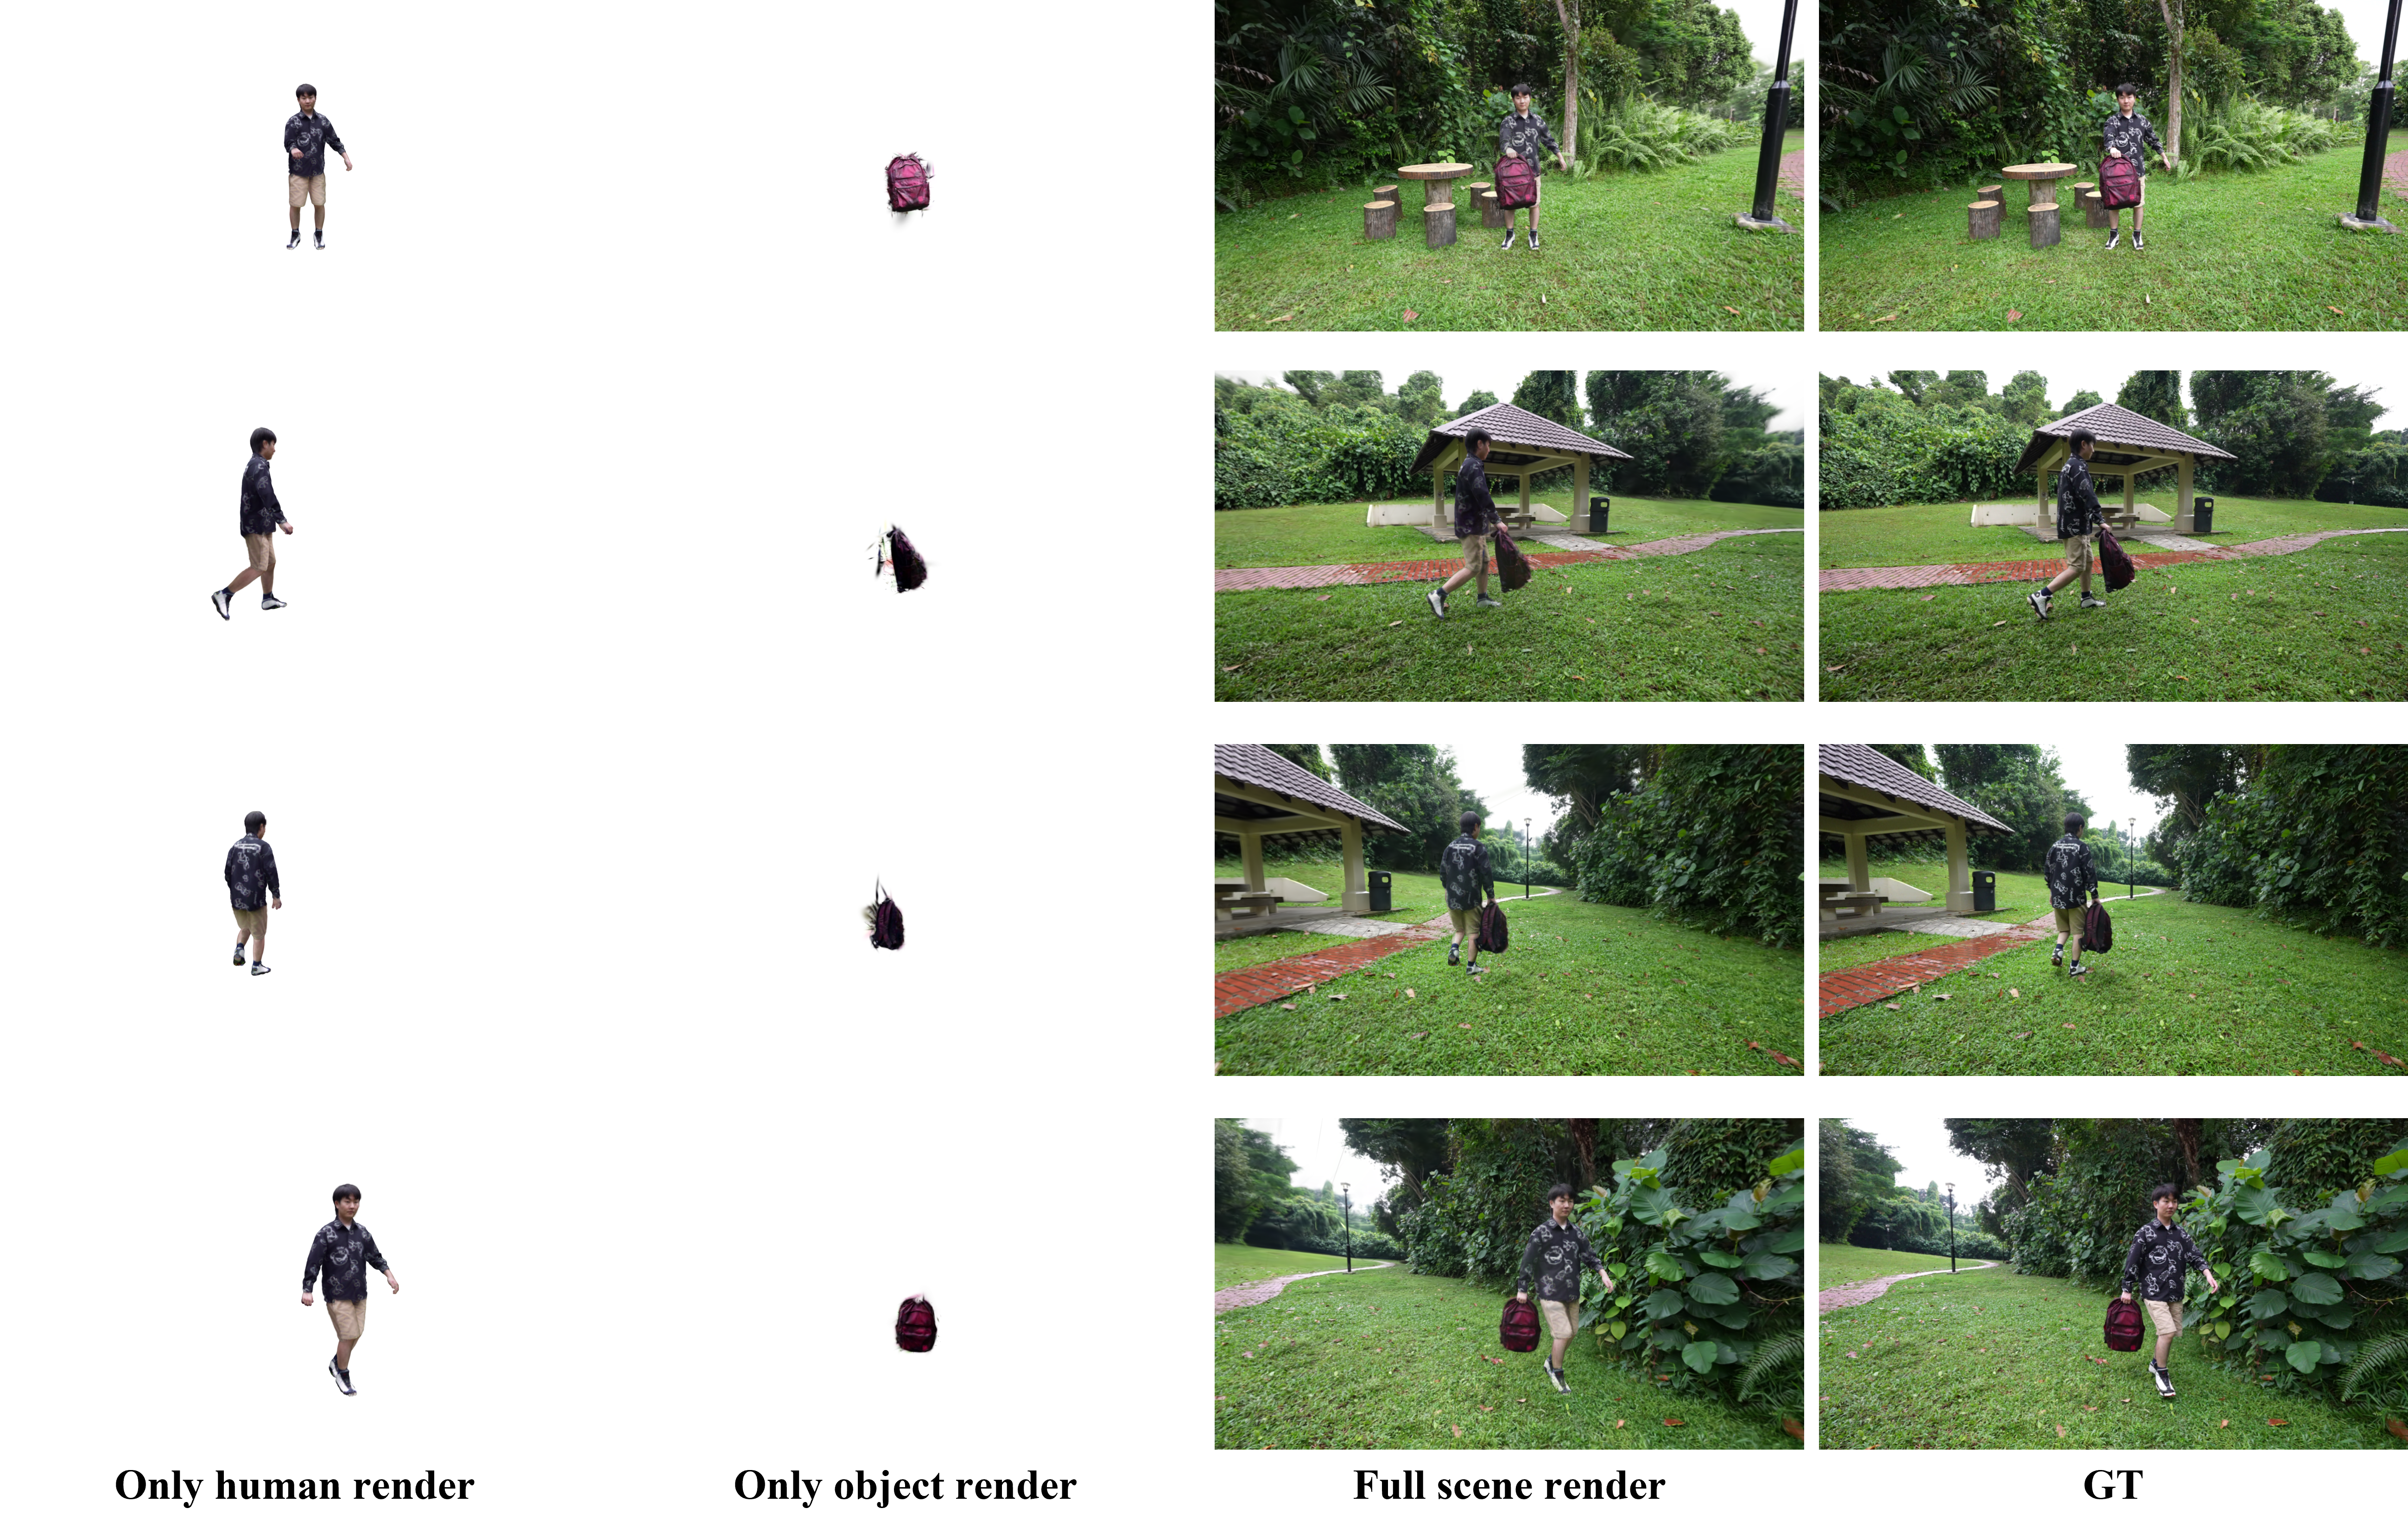
\includegraphics[width=\textwidth]{iclr2026/images/appendix/Appendix_1.png}}
    \vspace{-2mm}
    \caption{\textbf{Decomposed scene reconstruction.}
    Visualization of individual scene components demonstrating geometric integrity in occluded regions. From left to right: human-only rendering, object-only rendering, full scene rendering, and ground truth. Each row shows a different frame from the sequence, highlighting that both human and object maintain coherent geometry even during close contact and occlusion.}
    \label{fig:decomposed_render}
\end{figure*}

\subsection{Decomposed Visualization}
\textcolor{blue}{
\textbf{Component-level Reconstruction Quality.} 
To address concerns about reconstruction quality in occluded regions, we provide decomposed visualizations that isolate individual scene components. As shown in Figure~\ref{fig:decomposed_render}, we render the human and object separately to demonstrate that each component maintains geometric integrity even in regions with heavy occlusion or contact.}

\textcolor{blue}{
\textbf{Human-only Rendering (Column 1):} The isolated human reconstruction shows coherent body geometry throughout the sequence, including regions that were occluded by the object (backpack) in the original footage. This demonstrates that our hexplane-based human deformation successfully captures the complete body structure without artifacts from the interacting object.}

\textcolor{blue}{
\textbf{Object-only Rendering (Column 2):} The object is reconstructed as a distinct, stable entity with well-defined geometry. Unlike single-field approaches that often produce fused or melted geometry at contact points, our CHS-based object deformation maintains clear boundaries and structural consistency throughout the interaction.}

\textcolor{blue}{
\textbf{Full Scene Rendering (Column 3):} The combined rendering seamlessly integrates both components and closely matches the ground truth, confirming that our explicit modeling of human-object interactions through the HOI module enables accurate disentanglement while preserving realistic appearance.}

\textcolor{blue}{
These results validate that HOIGS does not simply overfit the combined RGB appearance but genuinely learns separate geometric representations for humans and objects. The clean separation at contact boundaries and the preservation of geometry in occluded regions demonstrate the effectiveness of our approach in handling complex interaction scenarios.
}
\subsection{Quantitative Evaluation of Human Pose Accuracy}

\begin{table*}[t]
\centering
\tiny
\setlength\tabcolsep{1.0pt}
\def\arraystretch{1.4} % Increased slightly for better separation of slashed values
\resizebox{\textwidth}{!}{%
\begin{tabular}{C{2.5cm}|C{3.2cm}C{3.2cm}C{3.2cm}C{3.2cm}}
\specialrule{.1em}{.05em}{.05em}

% -------- Part 1: First 4 Classes --------
\textbf{Model} &
\textbf{Backpack1} &
\textbf{Plasticcontainer1} &
\textbf{Plasticcontainer2} &
\textbf{Suitcase1} \\ \hline

ExAvatar & 
0.4196 / 0.4628 / 0.3687 & 
0.3875 / 0.4282 / 0.3563 & 
0.3094 / 0.3145 / 0.2897 & 
0.2654 / 0.2957 / 0.2505 \\

HOIGS (Ours) & 
0.4177 / 0.4539 / 0.3656 & 
0.2964 / 0.3344 / 0.2863 & 
0.2973 / 0.3120 / 0.2837 & 
0.2438 / 0.2649 / 0.2352 \\

\specialrule{.1em}{.05em}{.05em}

% -------- Part 2: Next 4 Classes --------
\textbf{Model} &
\textbf{Backpack2} &
\textbf{Plasticcontainer3} &
\textbf{Backpack3} &
\textbf{Trashbin} \\ \hline

ExAvatar & 
0.2690 / 0.3135 / 0.2488 & 
0.3293 / 0.3298 / 0.2970 & 
0.2177 / 0.2494 / 0.2092 & 
0.2294 / 0.2597 / 0.2156 \\

HOIGS (Ours) & 
0.2629 / 0.3068 / 0.2438 & 
0.3270 / 0.3265 / 0.2948 & 
0.2110 / 0.2380 / 0.2020 & 
0.2263 / 0.2550 / 0.2126 \\

\specialrule{.1em}{.05em}{.05em}

\end{tabular}%
}
\caption{
Unified quantitative evaluation on the BEHAVE dataset. The values in each cell correspond to \textbf{PA-MPJPE / PA-MPJPE (Hand/Forearm) / PA-PVE}. HOIGS consistently outperforms the baseline across these metrics, particularly in interaction-critical regions.
}
\label{tab:unified_comparison}
\end{table*}


\textcolor{blue}{
\textbf{Geometric Fidelity Analysis}. 
We acknowledge that rendering metrics alone are insufficient to fully validate the geometric fidelity of complex human–object interactions. To address this, we conducted additional evaluations on human pose accuracy using the BEHAVE dataset. We compare our method against ExAvatar using PA-MPJPE (Procrustes Aligned Mean Per Joint Position Error) and PA-PVE (Procrustes-Aligned Per Vertex Error).
}

\begin{figure*}[htb!]
\centerline{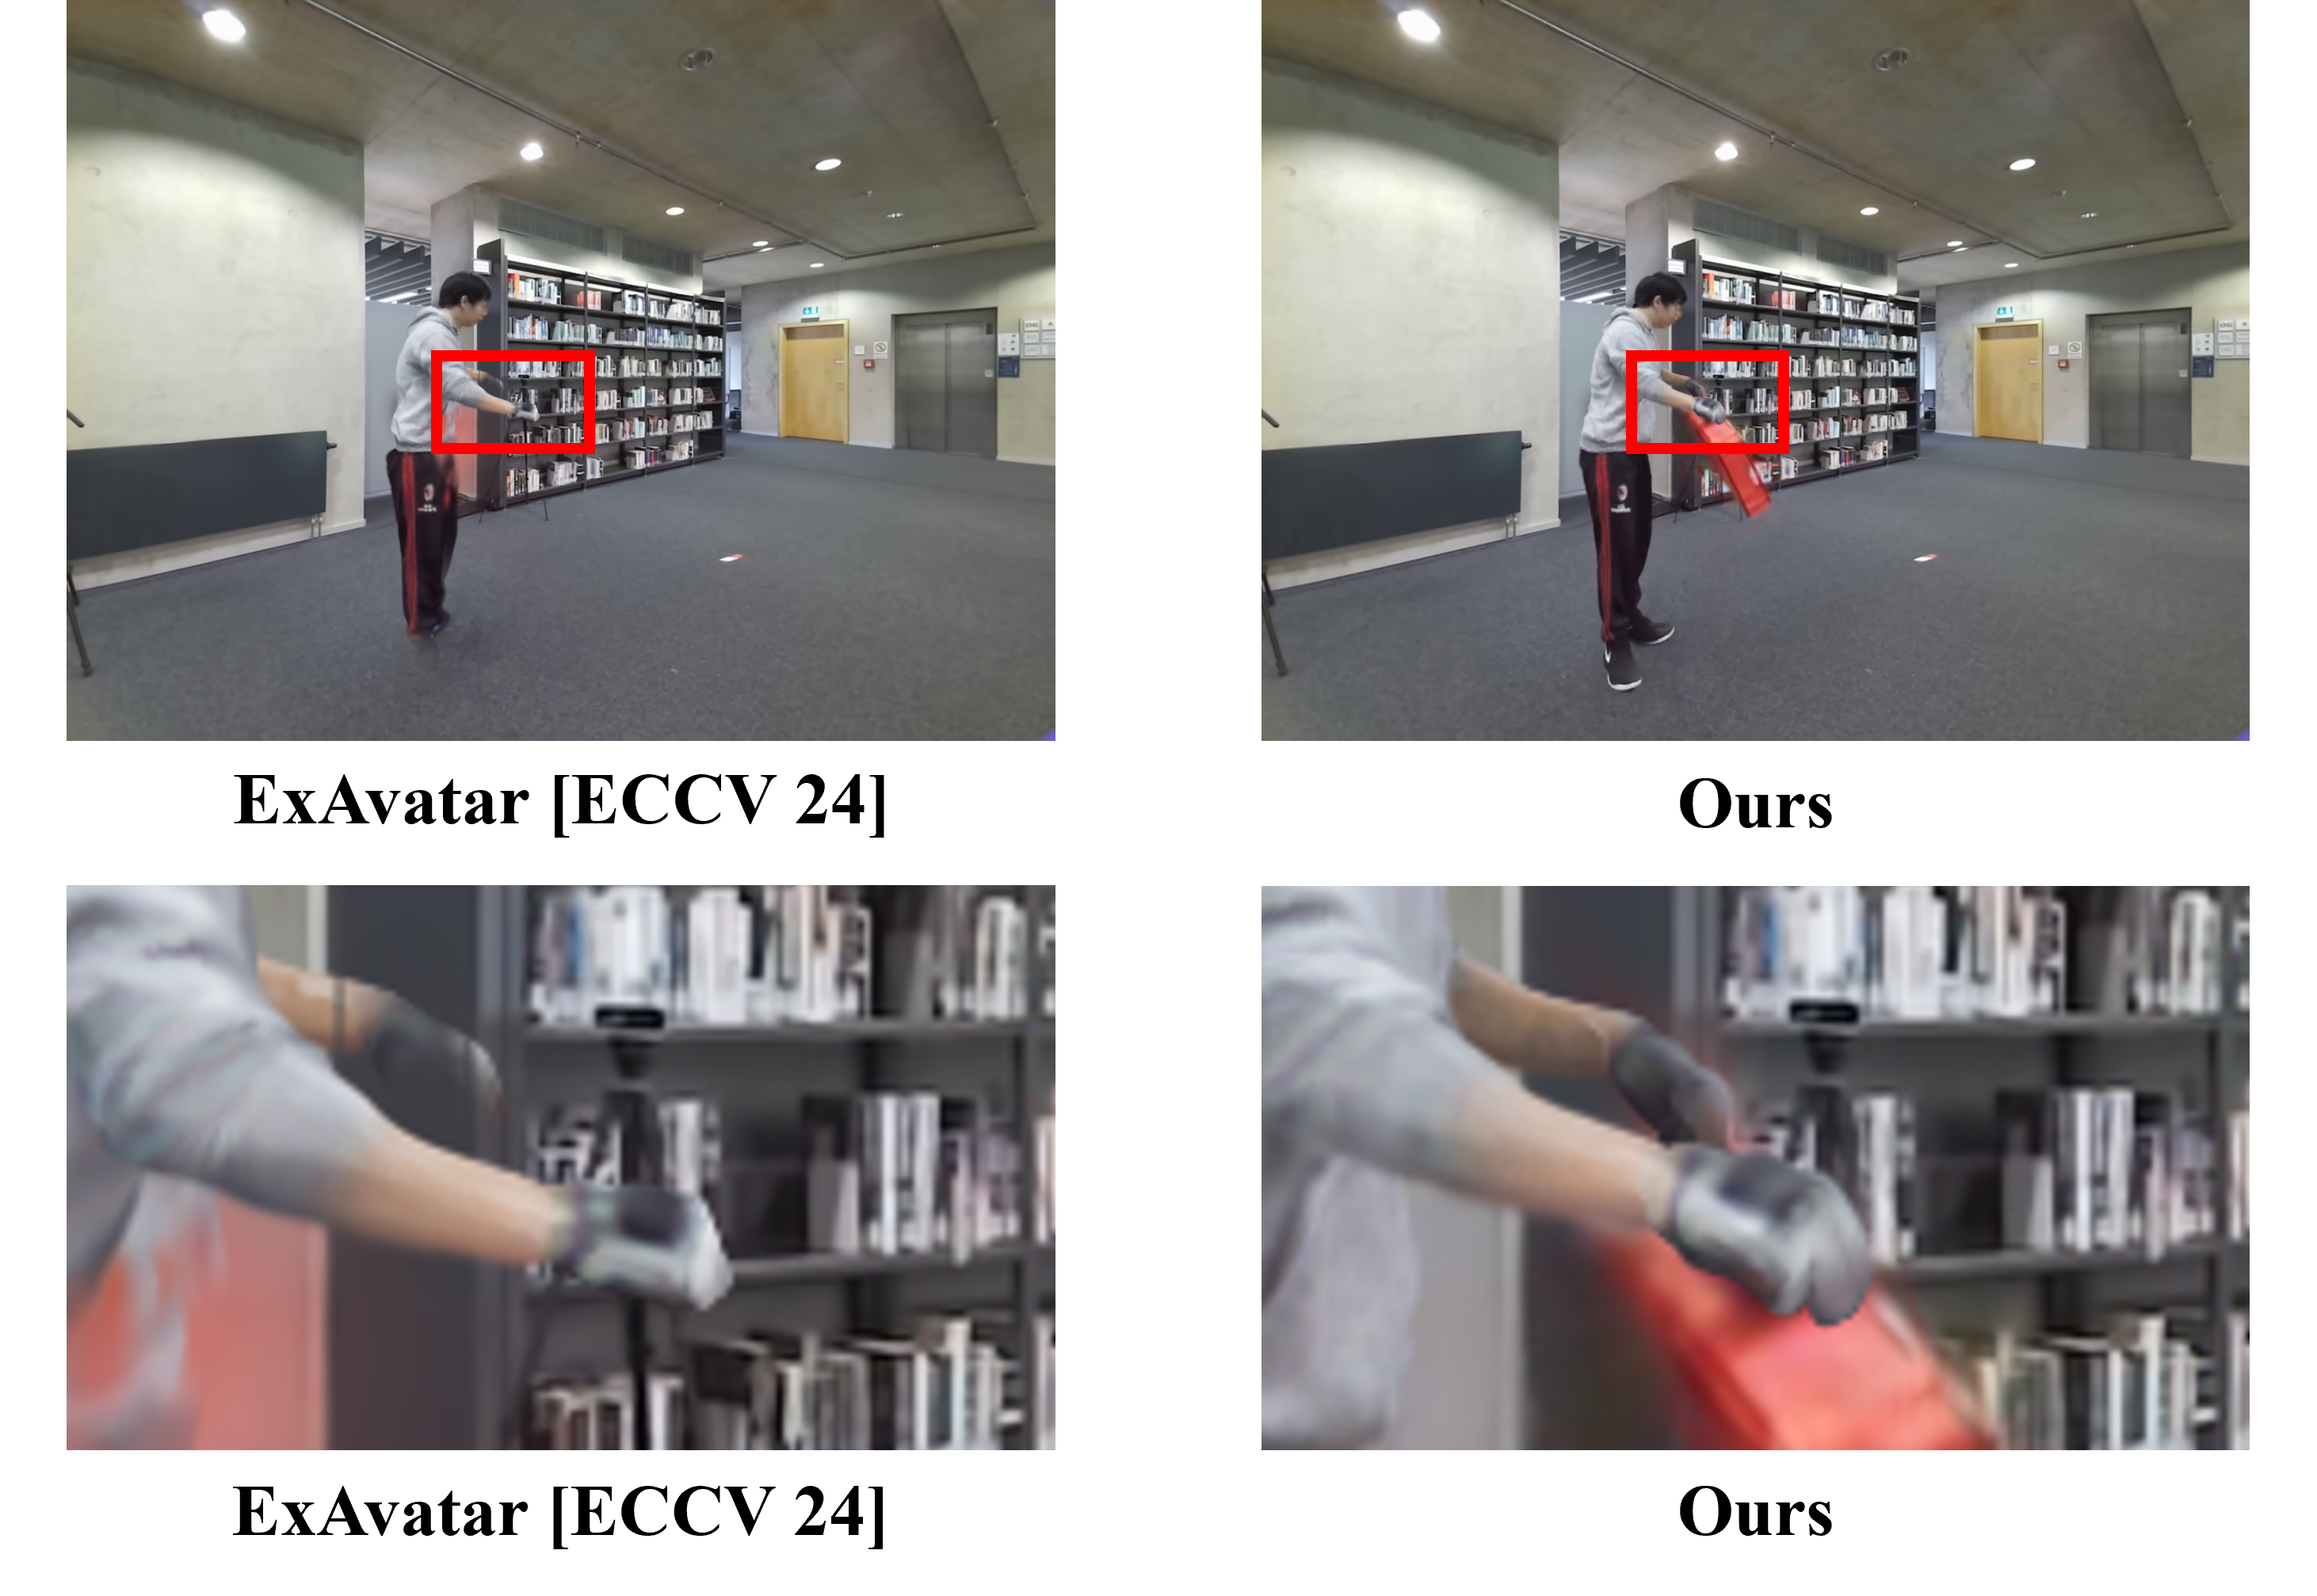
\includegraphics[width=\textwidth]{iclr2026/images/appendix/behave_refine.png}}
    \vspace{-2mm}
    \caption{\textbf{Qualitative comparison of human pose refinement on the BEHAVE dataset.}
    Visual comparison between ExAvatar and our method (HOIGS). The red boxes highlight the interaction regions (hands and objects). Our HOI module explicitly refines the hand and forearm poses by leveraging object motion features, leading to accurate contact modeling, whereas ExAvatar exhibits misalignment in these interaction-rich regions.}
    \label{appendix_behave_refine}
\end{figure*}


\textcolor{blue}{
\textbf{Effect of the HOI Module on Pose Refinement}.
Our method explicitly models the mutual dependency between the human and the object. The HOI module leverages a cross-attention mechanism to use object motion features as contextual cues to refine human features. Specifically, as described in Eq. 14 of the main paper, the module predicts refinement offsets $\Delta$SMPL-X for the body and hands. This capability allows the network to correct the human pose—even under partial occlusion—by inferring the likely body configuration from the object's trajectory.
}


\textcolor{blue}{
\textbf{Quantitative Results}.
Table \ref{tab:unified_comparison} summarizes the evaluation on the BEHAVE dataset. We report the average PA-MPJPE and PA-PVE across all test frames. Additionally, we provide a specific analysis for Hand and Forearm joints, which are the most critical regions for interaction tasks.
}
\textcolor{blue}{
As shown in Table \ref{tab:unified_comparison}, HOIGS consistently outperforms the baseline. Notably, we observe a larger performance gain in the \textbf{PA-MPJPE (Hand/Forearm joints)}. This indicates that our HOI module effectively refines the poses of interaction-related body parts, resulting in physically more accurate reconstructions compared to ExAvatar, which lacks mutual feedback between the human and the object. Please refer to the per-sequence detailed tables at the bottom of the appendix.}

\subsection{Sensitivity Analysis on External Modules}

\begin{table*}[t]
\centering
\small
\setlength\tabcolsep{1.0pt}
\resizebox{\textwidth}{!}{%
\begin{tabular}{C{4.3cm}|C{1.1cm}C{1.1cm}|C{1.1cm}C{1.1cm}|C{1.1cm}C{1.1cm}|C{1.1cm}C{1.1cm}|C{1.1cm}C{1.1cm}|C{1.1cm}C{1.1cm}|C{1.1cm}C{1.1cm}}
\specialrule{.1em}{.05em}{.05em}
\multirow{2}{*}{Method Combinations} &
\multicolumn{2}{c|}{\textbf{Backpack}} &
\multicolumn{2}{c|}{\textbf{Tennis}} &
\multicolumn{2}{c|}{\textbf{Suitcase}} &
\multicolumn{2}{c|}{\textbf{Playground}} &
\multicolumn{2}{c|}{\textbf{Dance}} &
\multicolumn{2}{c|}{\textbf{Lounge}} &
\multicolumn{2}{c}{\textbf{Average}} \\
& PSNR$\uparrow$ & LPIPS$\downarrow$
& PSNR$\uparrow$ & LPIPS$\downarrow$
& PSNR$\uparrow$ & LPIPS$\downarrow$
& PSNR$\uparrow$ & LPIPS$\downarrow$
& PSNR$\uparrow$ & LPIPS$\downarrow$
& PSNR$\uparrow$ & LPIPS$\downarrow$ 
& PSNR$\uparrow$ & LPIPS$\downarrow$ \\ \hline

Samurai + MetricV2
& 25.78 & 0.082 
& 27.12 & 0.108 
& 22.09 & 0.246 
& 25.23 & 0.103 
& 24.17 & 0.098 
& 30.97 & 0.048 
& 25.89 & 0.114 \\

Samurai + Video Depth Anything
& 25.85 & 0.080 
& 27.18 & 0.106 
& 22.15 & 0.241 
& 25.28 & 0.102 
& 24.22 & 0.096 
& 31.05 & 0.046 
& 25.96 & 0.112 \\

Samurai + DepthCrafter
& 25.72 & 0.088 
& 27.08 & 0.108 
& 22.06 & 0.249 
& 25.20 & 0.109 
& 24.08 & 0.099 
& 30.93 & 0.048 
& 25.85 & 0.117 \\

TrackAnything + MetricV2
& 25.72 & 0.086 
& 27.05 & 0.109 
& 22.03 & 0.246 
& 25.18 & 0.106 
& 24.15 & 0.100 
& 30.93 & 0.052 
& 25.84 & 0.116 \\

SAMv2 + Video Depth Anything
& 26.01 & 0.076 
& 27.38 & 0.103 
& 22.33 & 0.241 
& 25.47 & 0.100 
& 24.42 & 0.095 
& 31.20 & 0.041 
& 26.14 & 0.109 \\

MaskRCNN + MetricV2
& 25.33 & 0.099 
& 26.67 & 0.125 
& 21.66 & 0.257 
& 24.78 & 0.117 
& 23.69 & 0.110 
& 30.52 & 0.065 
& 25.44 & 0.129 \\

\specialrule{.1em}{.05em}{.05em}
\end{tabular}%
}
\caption{
Sensitivity analysis of HOIGS on the HOSNeRF dataset using different combinations of segmentation and depth estimation priors. The results demonstrate the robustness of our method, with consistent performance across various modern priors and strong performance even with older baselines (MaskRCNN).
}
\label{tab:sensitivity_analysis}
\end{table*}


\textcolor{blue}{
\textbf{Robustness to External Priors.}~
To address concerns regarding the reliance on external modules, we conducted a sensitivity analysis on the HOSNeRF dataset by evaluating our framework with various combinations of segmentation (e.g., Samurai~\cite{yang2024samurai}, SAMv2~\cite{ravi2024sam2}, MaskRCNN~\cite{massa2018mrcnn}, TrackAnything~\cite{yang2023track}) and depth estimation (e.g., Video Depth Anything~\cite{video_depth_anything}, MetricV2~\cite{hu2024metric3dv2}, DepthCrafter~\cite{hu2025-DepthCrafter}) models.~
As shown in Table~\ref{tab:sensitivity_analysis}, HOIGS maintains highly consistent performance (Avg PSNR 25.8--26.1) across different modern priors, demonstrating that our method is robust to variations in preprocessing quality.~
Notably, even when employing the standard, older baseline of MaskRCNN combined with MetricV2, our model achieves an average PSNR of 25.44.~
This performance remains significantly higher than the state-of-the-art human-centric baseline, ExAvatar (Avg PSNR 24.35), and the 4DGS baseline, Ex4DGS (Avg PSNR 17.97).
}


% \textcolor{blue}{
% \textbf{Robustness to External Priors.} 
% To address concerns regarding the reliance on external modules, we conducted a sensitivity analysis on the HOSNeRF dataset by evaluating our framework with various combinations of segmentation (e.g., Samurai, SAMv2, MaskRCNN, TrackAnything) and depth estimation (e.g., Video Depth Anything, MetricV2, DepthCrafter) models. 
% As shown in Table~\ref{tab:sensitivity_analysis}, HOIGS maintains highly consistent performance (Avg PSNR 25.8--26.1) across different modern priors, demonstrating that our method is robust to variations in preprocessing quality. 
% Notably, even when employing the standard, older baseline of MaskRCNN combined with MetricV2, our model achieves an average PSNR of 25.44. 
% This performance remains significantly higher than the state-of-the-art human-centric baseline, ExAvatar (Avg PSNR 24.35), and the 4DGS baseline, Ex4DGS (Avg PSNR 17.97).
% }

 
\subsection{Computational Complexity and Runtime Analysis}
\textcolor{blue}{
\textbf{Runtime Performance}.
We evaluate the computational efficiency of our method on the HOSNeRF dataset using a single NVIDIA H100 GPU. As shown in Table~\ref{tab:runtime_comparison}, our method achieves an inference speed of \textbf{44.27 FPS}. While this is slightly lower than 4DGS~\cite{wu20244d} (61.04 FPS), it remains comparable to Ex4DGS~\cite{lee2024fully} (46.38 FPS) and outperforms D3DGS~\cite{yang2024deformable} (37.79 FPS). This result confirms that the inclusion of the HOI attention mechanism does not create a significant bottleneck, allowing our method to comfortably support real-time applications.
}
\begin{table}[t] % Changed [h] to [t] or [ht] for better float placement
\centering
\small
\setlength\tabcolsep{8.0pt}
% Using resizebox to match your style
\resizebox{0.7\textwidth}{!}{%
\begin{tabular}{l|c|c}
\specialrule{.1em}{.05em}{.05em}
\textbf{Methods} & \textbf{Training Time} & \textbf{Inference Speed (FPS)} \\ \hline
4DGS~\cite{wu20244d} & 40 min & 61.04 \\
Ex4DGS~\cite{lee2024fully} & 2 hr 30 min & 46.38 \\
D3DGS~\cite{yang2024deformable} & 3 hr & 37.79 \\
E-D3DGS~\cite{bae2024per} & 2 hr & 54.71 \\ \hline
\textbf{HOIGS (Ours)} & 5 hr & 44.27 \\
\specialrule{.1em}{.05em}{.05em}
\end{tabular}%
}
\caption{
Runtime performance comparison on the HOSNeRF dataset. We report the approximate training time per scene and the inference speed in Frames Per Second (FPS). Our method maintains real-time performance ($>$30 FPS) despite the added complexity of interaction modeling.
}
\label{tab:runtime_comparison}
\end{table}

\textcolor{blue}{
\textbf{Complexity Analysis}.
The efficiency of our HOI module stems from the token-based architectural design. The cross-attention is computed between $M$ human part tokens (where $M=16$ is fixed) and $N$ object Gaussian tokens. Unlike standard self-attention which scales quadratically ($O(N^2)$), our cross-attention scales linearly ($O(M \cdot N)$) with respect to the number of object Gaussians. Furthermore, we utilize compact 32-dimensional embeddings for object motion features, which minimizes the memory footprint and matrix multiplication overhead during the forward pass.
}

\textcolor{blue}{
\textbf{Training Cost Justification}.
We acknowledge that our training time ($\sim$5 hours) is longer than the baselines. This is a deliberate trade-off to prioritize physical plausibility and interaction accuracy. Explicitly modeling mutual dependencies and backpropagating gradients through the attention mechanism requires more iterations. However, this cost is strictly confined to the offline training phase, ensuring that the final online user experience remains real-time.
}

\begin{table*}[t]
\centering
\small
\setlength\tabcolsep{1.0pt}
\resizebox{\textwidth}{!}{%
\begin{tabular}{l|C{1.1cm}C{1.1cm}|C{1.1cm}C{1.1cm}|C{1.1cm}C{1.1cm}|C{1.1cm}C{1.1cm}|C{1.1cm}C{1.1cm}|C{1.1cm}C{1.1cm}|C{1.1cm}C{1.1cm}}
\specialrule{.1em}{.05em}{.05em}
\multirow{2}{*}{Methods} &
\multicolumn{2}{c|}{\textbf{Backpack}} &
\multicolumn{2}{c|}{\textbf{Tennis}} &
\multicolumn{2}{c|}{\textbf{Suitcase}} &
\multicolumn{2}{c|}{\textbf{Playground}} &
\multicolumn{2}{c|}{\textbf{Dance}} &
\multicolumn{2}{c|}{\textbf{Lounge}} &
\multicolumn{2}{c}{\textbf{Average}} \\
& PSNR$\uparrow$ & LPIPS$\downarrow$
& PSNR$\uparrow$ & LPIPS$\downarrow$
& PSNR$\uparrow$ & LPIPS$\downarrow$
& PSNR$\uparrow$ & LPIPS$\downarrow$
& PSNR$\uparrow$ & LPIPS$\downarrow$
& PSNR$\uparrow$ & LPIPS$\downarrow$
& PSNR$\uparrow$ & LPIPS$\downarrow$ \\ \hline

MASt3R Prior
& 23.51 & 0.135
& 25.25 & 0.121
& 22.40 & 0.197
& 24.65 & 0.074
& 23.63 & 0.115
& 28.99 & 0.057
& 24.59 & 0.128 \\

Depth Recon Prior
& 21.63 & 0.142
& 25.65 & 0.122
& 22.13 & 0.230
& 25.24 & 0.103
& 24.08 & 0.123
& 28.95 & 0.095
& 25.36 & 0.136 \\

\hline
\textbf{Diffusion Prior (Ours)}
& 23.70 & 0.082
& 27.13 & 0.112
& 22.96 & 0.235
& 25.63 & 0.123
& 24.17 & 0.093
& 29.97 & 0.043
& 25.89 & 0.114 \\

\specialrule{.1em}{.05em}{.05em}
\end{tabular}%
}
\caption{
Quantitative ablation study on Object Priors using the HOSNeRF dataset. We evaluate the effectiveness of our Diffusion Prior against MASt3R and Depth Reconstruction priors.
}
\label{tab:prior_ablation}
\end{table*}

\subsection{Additional Ablation Studies}

\textcolor{blue}{
\textbf{Impact of Object Diffusion Prior.} 
To validate the effectiveness of our design choice, we investigate the impact of different geometric priors on the final reconstruction quality. We compare our proposed method, which utilizes a generative Diffusion Prior, against two alternative initialization strategies:\\
(1) MASt3R Prior: Initialization using MASt3R, a state-of-the-art dense matching and reconstruction model. \\
(2) Depth Reconstruction Prior: Initialization using standard monocular metric depth estimation.
}

\textcolor{blue}{
Table \ref{tab:prior_ablation} presents the quantitative comparison on the HOSNeRF dataset. 
Our method equipped with the Diffusion Prior achieves the highest average reconstruction quality (25.89 PSNR), outperforming the MASt3R prior (24.59 PSNR) and the Depth prior (25.36 PSNR).
While discriminative approaches like MASt3R or metric depth estimation rely heavily on visible cues, they often struggle to reconstruct accurate geometry in the presence of heavy occlusions, a common occurrence in human-object interaction scenarios (e.g., hands covering objects).
In contrast, the Diffusion Prior leverages generative knowledge to plausibly complete 3D geometry even in occluded or unseen regions. This holistic geometric initialization provides a more robust starting point for our Cubic Hermite Spline (CHS) deformation, leading to sharper rendering and more stable tracking throughout the dynamic sequence.
}

\subsection{Feature extraction}

\input{images_tex/appendix_object_feature}

\textbf{Object feature}.
%우리는 object feature를 추출하기 위해 key frame의 Gaussian에 대해 velocity vector와 임베딩 파라미터를 활용한다. 각 key frame의 velocity vector는 CHS에 적용되어 baseline deformation과 함께 HOI module의 입력 feature로 공동 최적화된다. 추가적으로 각 key frame의 Gaussian마다 29차원의 learnable parameter를 임베딩하며, 이 임베딩은 velocity vector와 결합되어 feature로 사용된다. CHS를 통해 interpolation된 Gaussian feature는 결합된 feature와 time 정보를 입력으로 받아 얕은 MLP layer를 거쳐 projection되며, 최종적으로 32차원의 feature를 형성한다.
As shown in Fig. \textcolor{blue}{\ref{appendix_objfeature}}(a), we extract object features by leveraging the velocity vectors and embedding parameters of Gaussians at key frames. As shown in Fig. \textcolor{blue}{\ref{appendix_objfeature}}(b), each key frame’s velocity vector is applied to the CHS and jointly optimized with the baseline deformation as input features for the HOI module. In addition, a 29-dimensional learnable parameter is embedded for each key frame Gaussian, which is concatenated with the velocity vector to form the feature representation. The interpolated Gaussian features produced by CHS are then combined with the concatenated feature and time information, and projected through a shallow MLP, resulting in a 32-dimensional feature vector.


\textbf{Human feature}.
Fig. \textcolor{blue}{~\ref{appendix_humanfeature}} illustrates the process of human feature extraction. 
We divide the SMPL-X model into 16 body parts and learn features corresponding to each part. 
Temporal features are sampled from the hexplane at SMPL-X vertices, where each feature at time $t$ is obtained based on the coordinates $(x_t, y_t, z_t)$. 
For each body part, the features of its associated vertices are averaged to form the part-specific representation $F_{\text{human}}$: 
\[
F_{\text{part}} = \frac{1}{N} \sum_{i \in \text{part}} f_i(x_t, y_t, z_t), \tag{10}
\]
where $N$ denotes the number of vertices belonging to the part. 
As a result, 16 part features, including head, torso, arms, and legs, are obtained and used as inputs to the HOI module. 
This design captures temporally varying dynamic representations while preserving semantically meaningful features for individual body parts.



\subsection{HOI module network detail}
As shown in Fig. \textcolor{blue}{\ref{appendix_HOINetwork}}, the proposed HOI module takes the time-varying features of humans and objects as inputs and explicitly models their interactions.
Let the human feature be denoted as $F_{\text{Human}} \in \mathbb{R}^{N_h \times d}$ and the object feature as $F_{\text{Object}} \in \mathbb{R}^{N_o \times d}$, 
where $N_h$ and $N_o$ are the numbers of feature tokens for human and object respectively, and $d$ is the feature dimension. 

To capture interdependencies between the two modalities, we apply a \textit{mutual-attention} mechanism. 
Specifically, queries ($Q$), keys ($K$), and values ($V$) are obtained via learnable linear projections:
\begin{equation}
Q_h = F_{\text{Human}}W_h^Q,\;\; K_o = F_{\text{Object}}W_o^K,\;\; V_o = F_{\text{Object}}W_o^V, \tag{11}
\end{equation}
\begin{equation}
Q_o = F_{\text{Object}}W_o^Q,\;\; K_h = F_{\text{Human}}W_h^K,\;\; V_h = F_{\text{Human}}W_h^V, \tag{12}
\end{equation}
where $W_h^Q, W_h^K, W_h^V, W_o^Q, W_o^K, W_o^V \in \mathbb{R}^{d \times d}$ are learnable projection matrices. 

Cross-attention is then computed in both directions: from human to object and from object to human. 
To enforce spatial priors, a distance mask $B \in \mathbb{R}^{N_h \times N_o}$ is added to the attention logits, where $B_{ij}$ encodes the relative distance between the $i$-th human token and the $j$-th object token. 
The resulting attention maps are defined as:
\begin{equation}
A_{h \leftarrow o} = \text{softmax}\!\left(\tfrac{Q_hK_o^\top}{\sqrt{d}} + B\right),\quad
A_{o \leftarrow h} = \text{softmax}\!\left(\tfrac{Q_oK_h^\top}{\sqrt{d}} + B^\top\right). \tag{13}
\end{equation}

Using these attention weights, the updated features are obtained as:
\begin{equation}
F'_{\text{Human}} = A_{h \leftarrow o} V_h,\quad
F'_{\text{Object}} = A_{o \leftarrow h} V_o. \tag{14}
\end{equation}

The updated human feature $F'_{\text{Human}}$ is then fed into a small MLP head to regress the refinement terms of SMPL-X parameters: 
\[
\Delta \text{SMPL-X} = \{\Delta \theta_{\text{body}},\; \Delta \theta_{\text{hand}}\;\}, \tag{15}
\]
where $\Delta \theta_{\text{body}}$ and $\Delta \theta_{\text{hand}}$ denote pose corrections for body and hands.
Similarly, the updated object feature $F'_{\text{Object}}$ is used to regress Gaussian-based object motion corrections:
\[
\Delta G_{\text{object}} \in \mathbb{R}^{N_o \times 3}, \tag{16}
\]
which represent displacement vectors applied to object Gaussians. 

In this way, the HOI module augments the baseline deformations (hexplane+LBS for humans and CHS for objects) with interaction-aware refinements, enabling accurate reconstruction of complex human--object interaction scenes.

\begin{figure*}[t!]
\centerline{\includegraphics[width=\textwidth]{images/appendix/human_feature.jpg}}
    \vspace{-2mm}
    \caption{\textbf{Human feature extraction.}
    }
    \label{appendix_humanfeature}
    \vspace{-5mm}
\end{figure*}

\subsection{Objective Function Details}
The overall loss function of our model is defined as follows:

\begin{equation}
L = \gamma L_{\text{object motion}} + \beta L_{\text{human}} + \sigma L_{\text{scene}} + L_{\text{depth}}, \tag{17}
\end{equation}

where $L_{\text{object motion}}$, $L_{\text{human}}$, and $L_{\text{scene}}$ correspond to losses for object motion, human modeling, and scene context, respectively. The weights $\gamma$, $\beta$, and $\sigma$ control the relative importance of each loss term and are specifically set to 1.0, 0.5, and 0.25, respectively. In our approach, these three terms are optimized simultaneously to consistently model the interactions between humans and objects.

\textbf{Human Loss details} \\
The $L_{\text{human}}$ term consists of losses related to human representation using the SMPL-X (\textcolor{blue}{\cite{pavlakos2019expressive}}) model. Specifically, it includes the reprojection error between the 3D human joint positions and detected 2D keypoints in images, a mesh-based face loss enhancing the consistency of facial geometry and texture, and a Laplacian regularization term. Additionally, there is an L1 loss ($L_{\text{smplx}}$) between the optimized SMPL-X parameters and the frame-wise initial SMPL-X parameters obtained by a regressor. These loss terms are directly adopted from previous methods such as ExAvatar (\textcolor{blue}{\cite{moon2024expressive}}), without modifications. For example, the face loss optimizes the consistency between rendered facial images and actual facial images, ensuring geometry-texture coherence. Laplacian regularization is applied to enhance the stability of human body shape. Further details can be found in the referenced research.

Formally, the human loss is given by:

\begin{equation}
L_{\text{human}} = L_{\text{kpt}} + L_{\text{face}} + L_{\text{reg}} + 0.1 \times L_{\text{smplx}}, \tag{18}
\end{equation}


\begin{figure*}[t!]
\centerline{\includegraphics[width=0.6\textwidth]{images/appendix/HOINetwork.jpg}}
    \vspace{-2mm}
    \caption{\textbf{Detailed HOI network.}
    The proposed architecture for estimating human-object interactions, leveraging features from human body parts and object Gaussian representations. The model takes as input human part features and per-Gaussian object features, processes them through bidirectional attention mechanisms to incorporate mutual contextual information, and outputs predictions for SMPL-X parameters per body part along with offset adjustments for object Gaussian centers.}
    \label{appendix_HOINetwork}
    \vspace{-5mm}
\end{figure*}
\textbf{Scene Loss details}\\
The $L_{\text{scene}}$ term is a photometric loss focusing on the background regions of the entire scene, following the image similarity-based loss used in existing 3D Gaussian Splatting (\textcolor{blue}{\cite{kerbl20233d}}) (3DGS) methods. Specifically, a pre-trained human/object segmentation model is employed to mask out human and object regions in the images, optimizing the background Gaussians for the remaining pixels only. This involves minimizing the difference between the rendered result and the background pixels excluding the segmented human and object areas. Occlusions frequently occur during interactions between human hands and objects, causing inconsistencies in masks. By optimizing humans, objects, and backgrounds simultaneously, our method effectively mitigates these boundary inconsistencies.

The scene loss is explicitly defined as:

\begin{equation}
L_{\text{scene}} = 0.8 \times L_1(I_{\text{gt}}, I_{\text{render}}) 
+ 0.2 \times L_{\text{D-SSIM}}(I_{\text{gt}}, I_{\text{render}}), \tag{19}
\end{equation}

\textbf{Object Loss details} \\
The $L_{\text{object}}$ term is a photometric loss that focuses exclusively on the object regions within the scene. We render only the segmented object areas and compute the loss solely on these regions. A pre-trained object segmentation model is employed to isolate object masks in the input images. The object loss encourages accurate reconstruction and appearance consistency for moving objects, which often undergo significant deformation and motion. By supervising only the object regions, this loss helps to refine the geometry and texture of the object-specific Gaussians without being influenced by background or human-related elements.

The object loss is defined as:
\begin{equation}
L_{\text{object motion}} = 0.8 \times L_1(I_{\text{gt}}, I_{\text{obj}}) 
+ 0.2 \times L_{\text{D-SSIM}}(I_{\text{gt}}, I_{\text{obj}}). \tag{20}
\end{equation}


 




\end{document}
